\documentclass[handout]{beamer}
%
%\mode<presentation>
%{
  \usetheme{Copenhagen} %type de présentation
  %\usecolortheme{blue}% couleur

  %\setbeamercovered{transparent} %laisse le texte à paraître en gris
%}
\usepackage[T1]{fontenc}
\usepackage[utf8]{inputenc}
\usepackage{lmodern}
\usepackage[frenchb]{babel}
\usepackage{amsmath}
\usepackage{amsfonts}
\usepackage{amssymb}


\frenchspacing

\allowdisplaybreaks %?
\let\Tiny=\tiny %pour enlever message erreur: Font shape `OT1/cmss/m/n? in size <4> not available
                %(Font) size <5> substituted on input line...

%\beamerdefaultoverlayspecification{<+->}


%-----------------------------------------------------------------------------------------------------------------
\title{Solitons et cosmologie, ou un exemple de symétrie et de beauté intersidérale}
\subtitle{Conférence du vendredi}
\author{Éric Dupuis}
\institute{Université de Montréal, département de physique des particules}
\date{XX-XX-2014}


%-----------------------------------------------------------------------------------------------------------------

\begin{document}

%titre
\begin{frame}
\titlepage
\end{frame}
%

\section*{}
\begin{frame}
\tableofcontents
\end{frame}

%-----------------------------------------------------------------------------------------------------------------
\section{Solitons - Appareillage mathématique }


\subsection{Équation d'ondes et soliton}
%eq d'onde
\begin{frame}
\frametitle{Équation d'ondes}
\begin{itemize}
\item  champ scalaire défini dans $\mathbb{R}^n$: $\phi(\vec{x},t)$\\
\end{itemize}
\begin{block}{équation d'onde}
\begin{equation}
\frac{1}{c^2}\frac{\partial^2 \phi}{\partial t^2} - \nabla^2 \phi = \square \phi = 0 
\end{equation}
\textit{Deux propriétés étudiées dans les solutions $\phi$}
\begin{itemize}
\item Forme et vitesse de l'onde conservées\\
\item Deux ondes retrouvent asymptotiquement leur forme et vitesse\\
\end{itemize}
\end{block} 
\end{frame}

%potentiel de solitons
\begin{frame}
\begin{enumerate}
\item Équation d'onde: V=0
\end{enumerate}

\begin{block}{Potentiels différents - Équations du mouvements modifiées}
\begin{enumerate}

\item terme dispersif: $\square\phi +$ \boldmath $m^2 \phi $ \unboldmath  = 0 (Klein-Gordon)\\
\begin{enumerate}
\item onde plane: $k^2 \rightarrow k^2+m^2$

\end{enumerate}
\item terme non-linéaire: $\phi^3$ \\
\end{enumerate}
\end{block}
En s'éloignant de l'équation d'onde, les deux propriétés peuvent être conservées: ondes solitaires et solitons 

\end{frame}

%photo Russell pour le plaisir
\begin{frame}
Sur sa monture, John Russell poursuit sa destinée qui le mène vers l'onde solitaire
\begin{columns}
    \begin{column}{.5\linewidth}
   \begin{figure}[0.3\textwidth]
    % 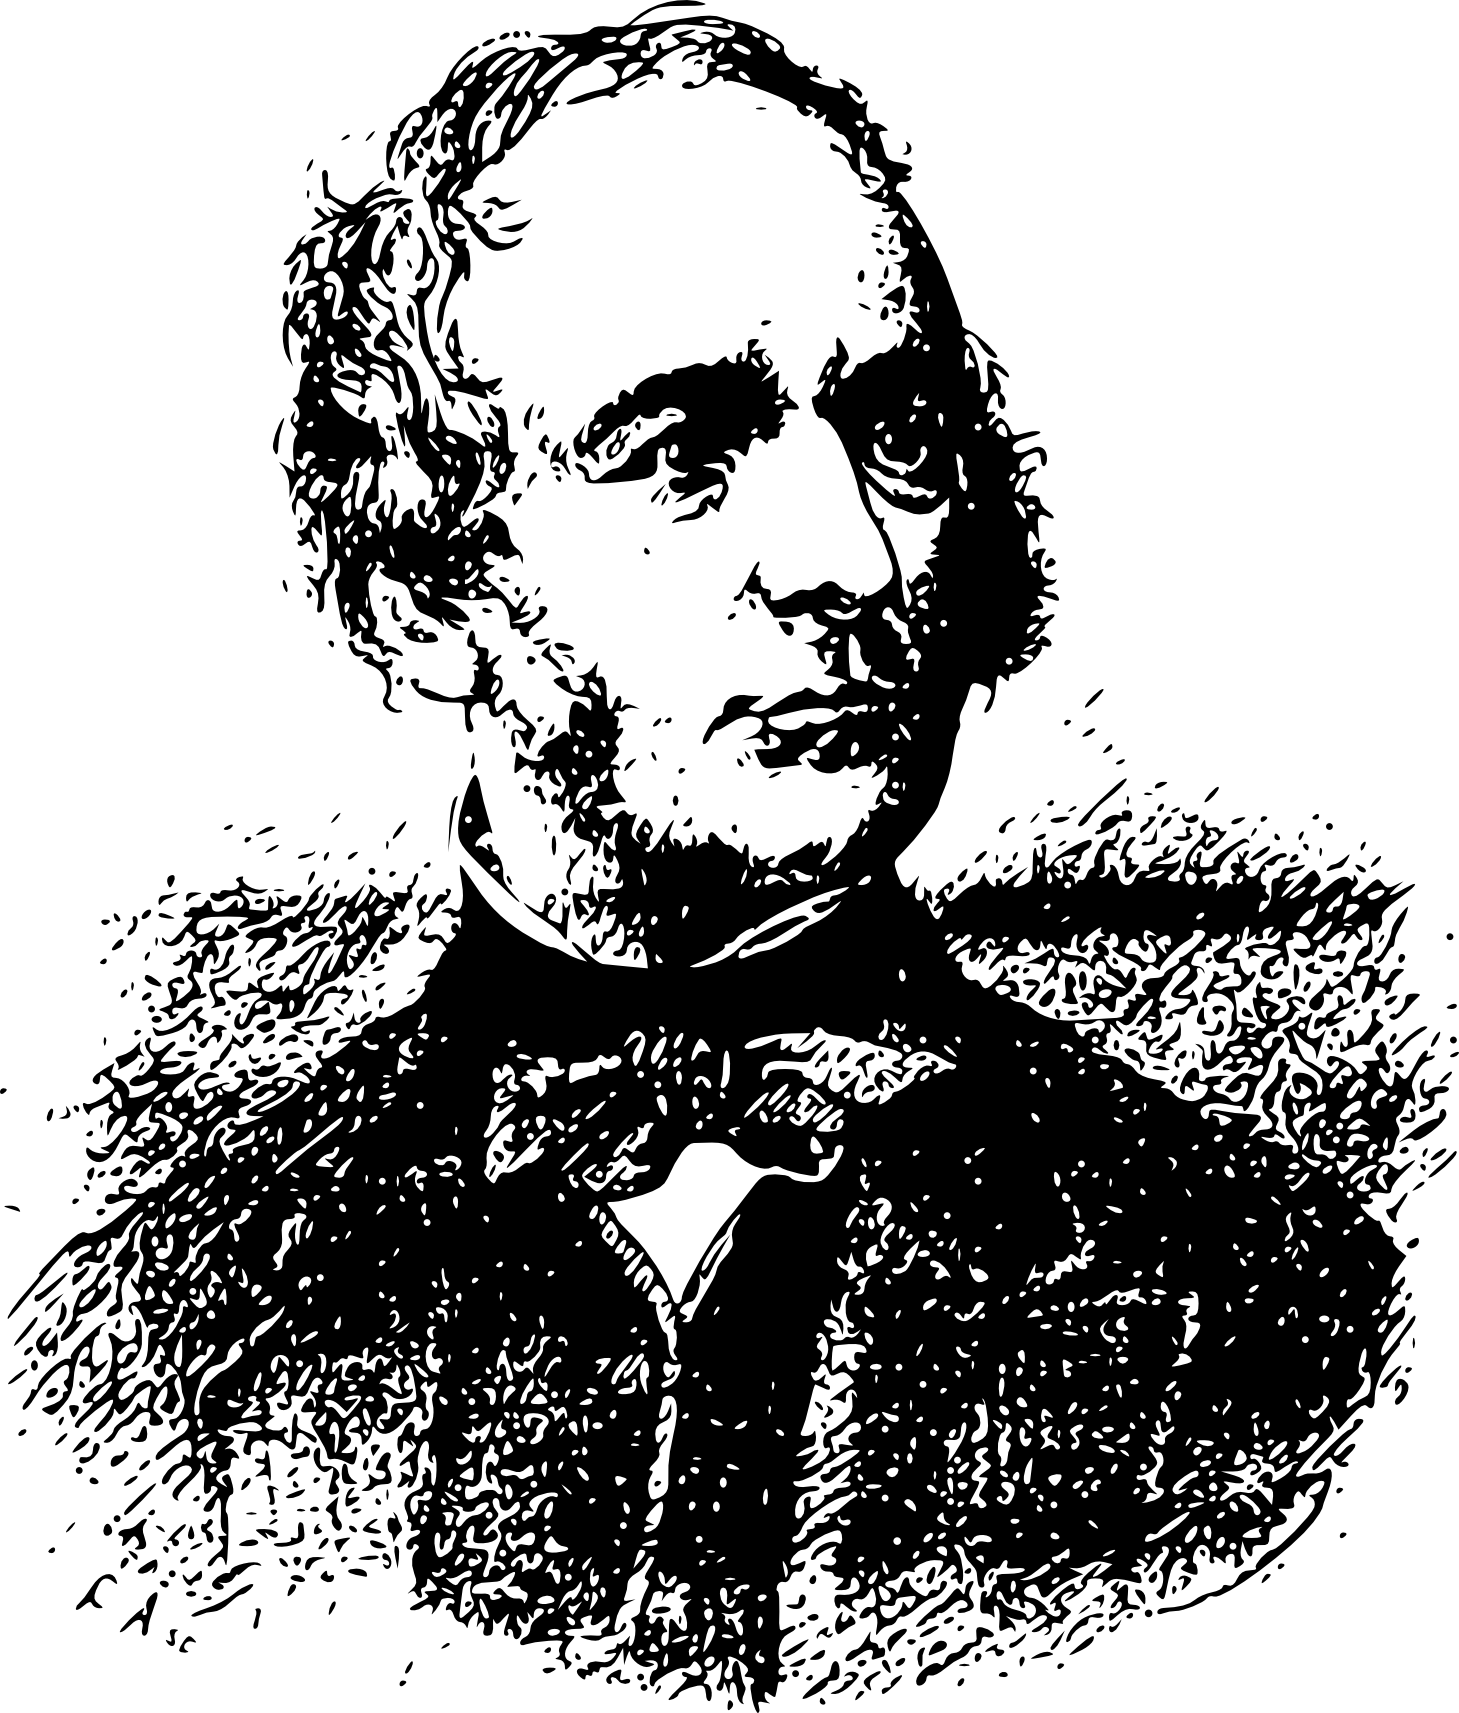
\includegraphics[scale=0.25]{russell.png}
    \end{figure}
    \end{column}
    \begin{column}{.5\linewidth}
    \begin{figure}[0.3\textwidth]
    % 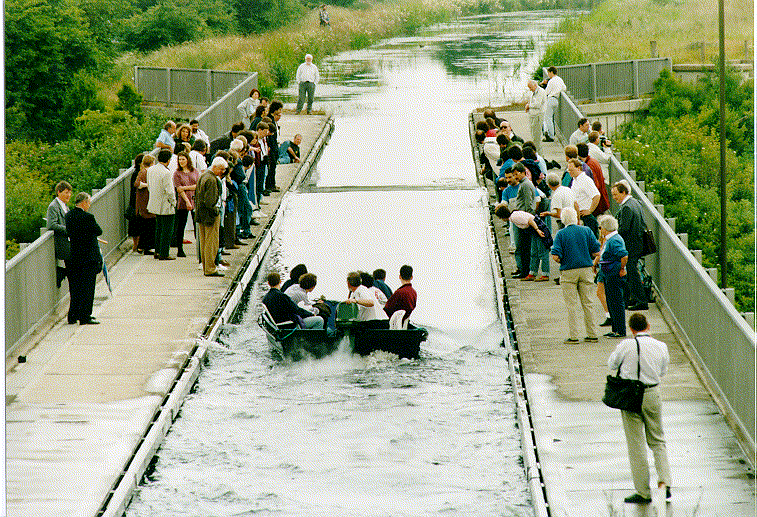
\includegraphics[scale=0.25]{soliton1b.png}
    \end{figure}
    \end{column}
  \end{columns}
\end{frame}


\begin{frame}
 \begin{columns}
    \begin{column}{.5\linewidth}
       \begin{figure}[0.3\textwidth]
    % 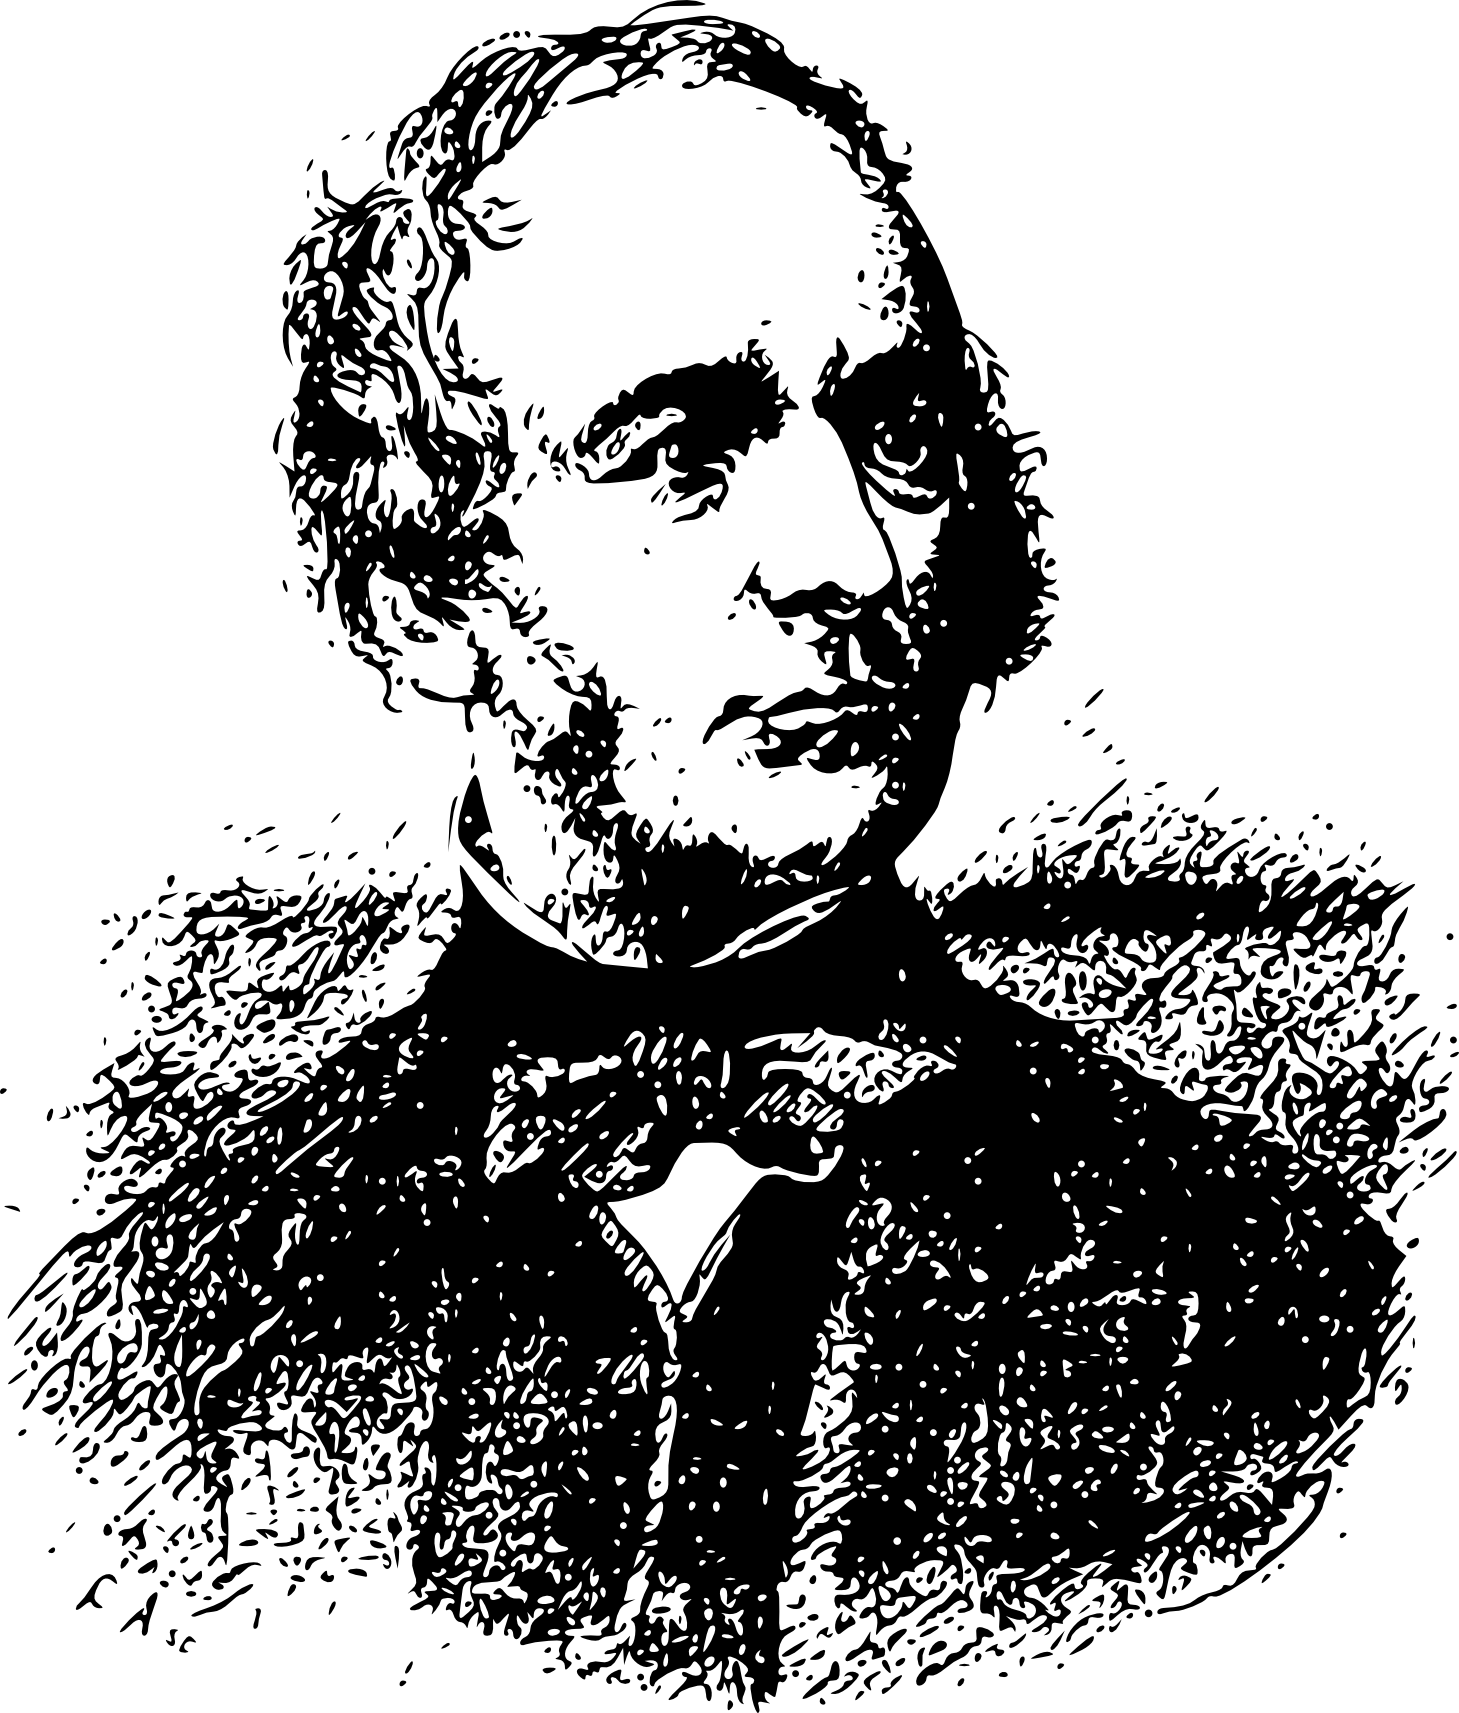
\includegraphics[scale=0.25]{russell.png} %densité d'énergie
    \end{figure}
    \end{column}
    \begin{column}{.5\linewidth}
	\begin{enumerate}
	\item Densité d'énergie d'un soliton $\epsilon(x,t)$: localisée dans l'espace
	\item $E[\phi] = \int{dxdt (\mathcal{H}[\phi])} = \int{dxdt [\frac{1}{2} \partial_x \phi (\partial_x \phi)^* +V]}$
	\item Énergie finie:
	\begin{enumerate}
	\item  $\lim\limits_{x \to \pm\infty}\partial_x E =0$
	\item  $\lim\limits_{x \to \pm\infty} \phi[x] = g^{(i)}$
	
	\end{enumerate}	
	\end{enumerate} 
    \end{column}
  \end{columns}
\end{frame}







\subsection{Formalisme Lagrangien}
\begin{frame}
\frametitle{Formalisme Lagrangien}
\begin{enumerate}
\item Potentiel défini pour toutes valeurs possibles de $\phi$: V($\phi$) \\
\item Notation covariante:
\begin{enumerate}
\item $x^\mu = (x^0,\vec{x})$
\item $x^0 = ct ; x^{1,2,3} = x,y,z$
\item $x^\mu = \eta^{\nu\mu} x_\nu$ métrique
\end{enumerate}
\item \textit{Action}: $S[\phi] = \int{dt (L[\phi])} = \int{dt dx^n (\mathcal{L}[\phi])}$ \\
\begin{enumerate}
\item Principe d'Hamilton: $\phi_0$ | action minimisée \\
\item Premier ordre nul pour un minimum d'action \\
\end{enumerate}
\item  $\mathcal{L}[\phi]$ = $\frac{1}{2} \partial_\mu \phi (\partial^\mu \phi)^* -V$\\
\item \textit{Euler-Lagrange:} $\partial_\mu \left(\frac{\mathcal{L}}{\partial(\partial_\mu\phi)}\right) = \frac{\partial\mathcal{L}}{\partial\phi}$
\begin{enumerate}
\item V=0 $\rightarrow \square\phi=0$
\end{enumerate}
\end{enumerate}
\end{frame}

\subsection{Kink}
\begin{frame}
\frametitle{Kink: cas de figure typique}
\begin{block}{Potentiel d'ordre 4}

 \begin{columns}
    \begin{column}{.5\linewidth}
    \begin{enumerate}
    \item deux minimums absolus
    \item ...
	\end{enumerate}      
    \end{column}
    \begin{column}{.5\linewidth}
    $V(\phi) = \frac{\lambda}{4}(|\phi|^2 -\frac{m^2}{\lambda})^2$
    \begin{figure}
     %\includegraphics[scale=0.5]{boom.jpg}
    \end{figure}
    \end{column}
  \end{columns}

\end{block}
$\mathcal{L} = \frac{1}{2}(\partial_x \phi)^2 - V $ \\
$\rightarrow \phi'' = \lambda \phi^3 - m^2 \phi$ \\
\end{frame}


\begin{frame}

\end{frame}


\begin{frame}
\begin{enumerate}
\item $\phi \rightarrow \phi(x,t)$: 1+1 dimensions
\item onde solitaire: solution statique
\end{enumerate}
\end{frame}


%-----------------------------------------------------------------------------------------------------------------
\section{Symétrie - Modèles de l'univers }
\begin{frame}
Thank you for your attention!
\end{frame}




\section{Cosmologie -  }

\section{Quotidien en cosmologie théorique des particules}
\begin{frame}
%potentiel avec lequel on travaille
\begin{block}{Potentiel à deux champs $\phi(x,t)$ et $\psi(x,t)$}
\begin{equation*}
V(\phi,\psi)=(\psi^2-\delta_1)(\psi^2-1)^2+\frac{\alpha}{\psi^2+\gamma}[(\phi^2-1)^2 - \frac{\delta_2}{4}(\phi-2)(\phi+1)^2] 
\end{equation*}
\begin{enumerate}
\item 1+1 dimensions (x,t) mais on cherche une solution statique
\item Beaucoup de paramètres: $\alpha, \gamma, \delta_1, \delta_2$
\item Les champs sont couplés
\end{enumerate}
\end{block}
\end{frame}

\begin{frame}
Pourquoi bâtir un potentiel comme ça en premier lieu?!?!\\


\begin{columns}
    \begin{column}{.5\linewidth}
   \begin{figure}[0.3\textwidth]
    % \includegraphics[scale=0.25]{potpsi.png}
    \end{figure}
   $\delta_1 \rightarrow$ contrôle du minima central\\
    Potentiel d'ordre 6, CLASSIQUE!\\    
    \end{column}
    \begin{column}{.5\linewidth}
    \begin{figure}[0.3\textwidth]
     %\includegraphics[scale=0.25]{potphi.png}
    \end{figure}
   $\delta_2 \rightarrow$ contrôle de la séparation entre minimum \\
    \end{column}
  \end{columns}
 $\alpha$: importance 2ème terme \\
 $\gamma$: importance couplage \\
\end{frame}

\end{document}